\documentclass{standalone}
\usepackage{tkz-fct}
\usepackage{tkz-euclide}
\usepackage{amsmath}
\usepackage{color}
\renewcommand*\familydefault{\sfdefault}
\usepackage{sansmath}
\sansmath
\definecolor{gray75}{gray}{0.75}
\begin{document}
 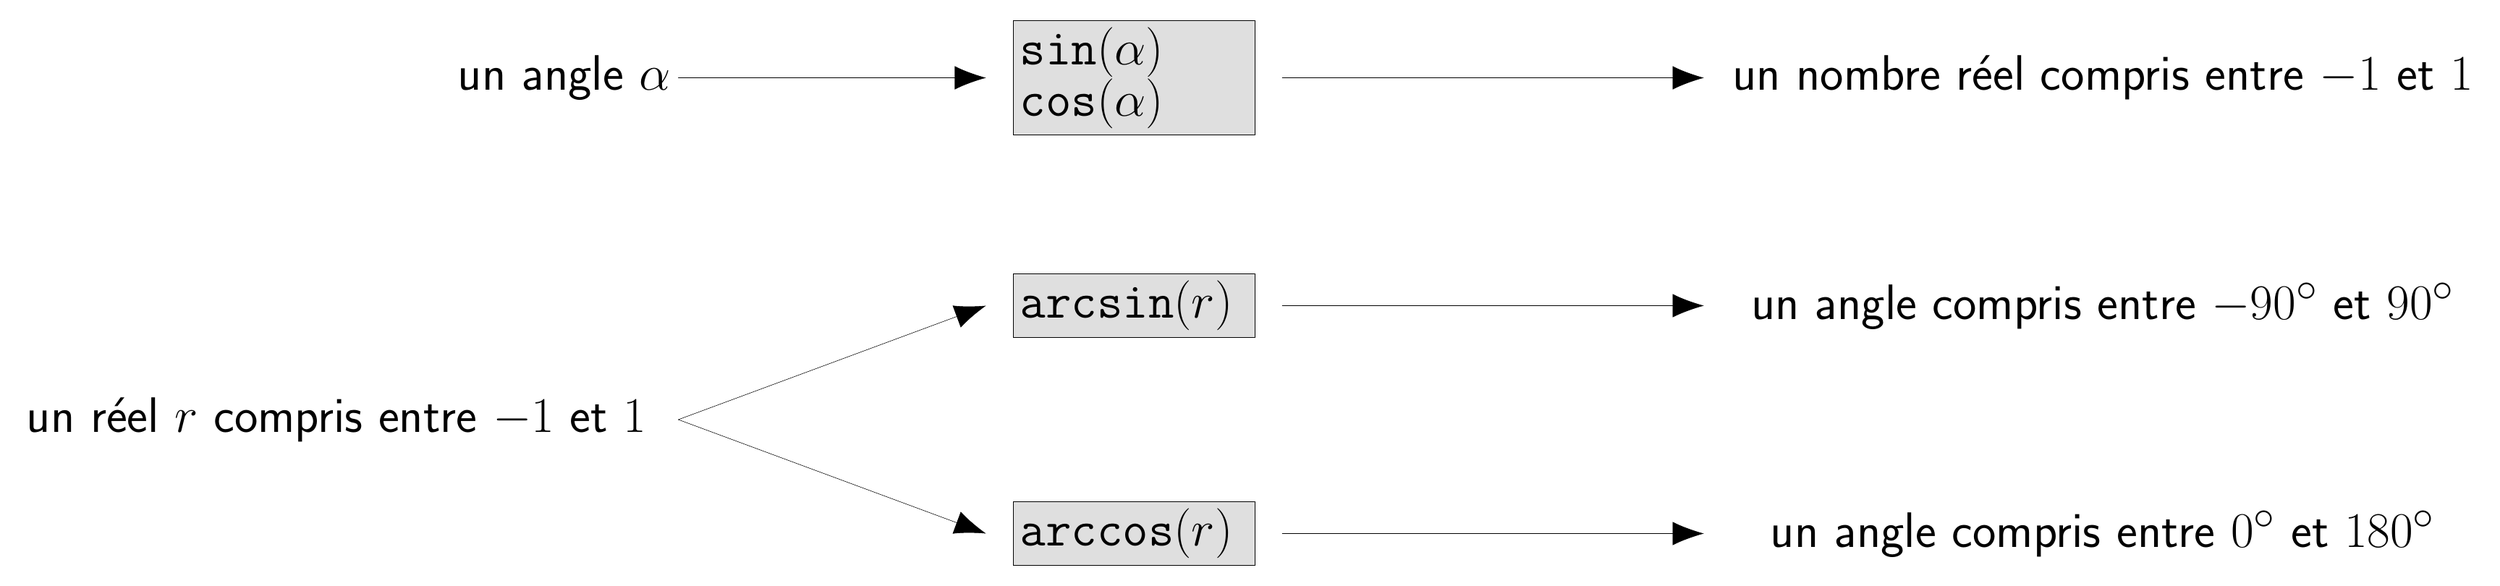
\begin{tikzpicture}[scale=2]
  \tikzset{vector style/.style={>={Latex[scale=4]},->}}
  \tkzDefPoints{-4/2/A,-1.3/2/B}

  \tkzDrawSegment[vector style](A,B)
  \tkzDefPoints{1.3/2/A,5/2/B}

  \tkzDrawSegment[vector style](A,B)
\tkzText(-5,2){\Huge un angle $\alpha$}

\tkzText[draw, fill=gray!25,text width=4cm](0,2){\centering{\Huge$\texttt{sin}(\alpha)$  $\texttt{cos}(\alpha)$}}

\tkzText(8.5,2){\Huge un nombre réel compris entre $-1$ et $1$}

\begin{scope}[yshift=-2cm]
  \tkzDefPoints{-4/1/A,-1.3/2/B}

  \tkzDrawSegment[vector style](A,B)
  \tkzDefPoints{1.3/2/A,5/2/B}

  \tkzDrawSegment[vector style](A,B)
  \tkzDefPoints{-4/1/A,-1.3/0/B}

  \tkzDrawSegment[vector style](A,B)
  \tkzDefPoints{1.3/0/A,5/0/B}

  \tkzDrawSegment[vector style](A,B)
\tkzText(-7,1){\Huge un réel $r$ compris entre $-1$ et $1$}

\tkzText[draw, fill=gray!25,text width=4cm](0,2){\centering{\Huge $\texttt{arcsin}(r)$}}

\tkzText(8.5,2){\Huge un angle compris entre $-90^{\circ}$ et $90^\circ$}

\tkzText[draw, fill=gray!25,text width=4cm](0,0){\centering{\Huge $\texttt{arccos}(r)$}}

\tkzText(8.5,0){\Huge un angle compris entre $0^{\circ}$ et $180^\circ$}
\end{scope}

\end{tikzpicture}
\end{document}
